%%%%%%%%%%%%%%%%%%%%%%%%%%%%%%%%%%%%%%%%%
% Vertical Line Title Page 
% LaTeX Template
% Version 1.0 (27/12/12)
%
% This template has been downloaded from:
% http://www.LaTeXTemplates.com
%
% Original author:
% Peter Wilson (herries.press@earthlink.net)
%
% License:
% CC BY-NC-SA 3.0 (http://creativecommons.org/licenses/by-nc-sa/3.0/)
% 
% Instructions for using this template:
% This title page compiles as is. If you wish to include this title page in 
% another document, you will need to copy everything before 
% \begin{document} into the preamble of your document. The title page is
% then included using \titleGM within your document.
%
%%%%%%%%%%%%%%%%%%%%%%%%%%%%%%%%%%%%%%%%%

%----------------------------------------------------------------------------------------
%	PACKAGES AND OTHER DOCUMENT CONFIGURATIONS
%----------------------------------------------------------------------------------------

\documentclass{article}

\usepackage{siunitx} % Provides the \SI{}{} and \si{} command for typesetting SI units
\usepackage{graphicx} % Required for the inclusion of images
\usepackage{natbib} % Required to change bibliography style to APA
\usepackage{amsmath} % Required for some math elements 
\usepackage{textcomp} % Required for the degree symbol
\usepackage[titletoc,title]{appendix} % fancy appendices
\usepackage{float} % Figure placement
\usepackage{geometry}
\usepackage{bm} % Bold bold math
\usepackage{nicefrac} % In-line fractions
\usepackage{tikz} % fancy diagrams
\usepackage{enumitem} % List sub numbers
\setlist[enumerate]{label*=\arabic*.}


\newcommand*{\plogo}{\fbox{$\mathcal{PL}$}} % Generic publisher logo
\renewcommand*\descriptionlabel[1]{\hspace\leftmargin$#1$}
\numberwithin{equation}{section}
\graphicspath{ {images/} }

%----------------------------------------------------------------------------------------
%	TITLE PAGE
%----------------------------------------------------------------------------------------

\newcommand*{\titleGM}{\begingroup % Create the command for including the title page in the document
\hbox{ % Horizontal box
\hspace*{0.2\textwidth} % Whitespace to the left of the title page
\rule{1pt}{\textheight} % Vertical line
\hspace*{0.05\textwidth} % Whitespace between the vertical line and title page text
\parbox[b]{0.75\textwidth}{ % Paragraph box which restricts text to less than the width of the page
\thispagestyle{empty}

{\noindent\Huge\bfseries Project Proposal}\\[2\baselineskip] % Title
{\large \textit{September 27, 2016}}\\[4\baselineskip] % Tagline or further description
{\large \textsc{City of Surrey Adaptive Signal Control Pilot: \\ 72 Avenue Through Newton Analysis}} % Date

\vspace{0.5\textheight} % Whitespace between the title block and the publisher
{\noindent 
	\textbf{Prepared by:} Team 7 \\ \hspace*{0.1\textwidth} % Whitespace between the vertical line and title page text
	\textit{Mak, Angelina (36741122) \\ \hspace*{0.1\textwidth} % Whitespace between the vertical line and title page text
		Russell, Alex (24645111) \\ \hspace*{0.1\textwidth} % Whitespace between the vertical line and title page text
		Shayesteh, Sadra (44781128) \\ \hspace*{0.1\textwidth} % Whitespace between the vertical line and title page text
		Soni, Darshan (46630125) \\ \hspace*{0.1\textwidth} % Whitespace between the vertical line and title page text
		Vibe, Christopher (51145126)} 
}\\[\baselineskip] % Publisher and logo
}}
\endgroup}

%----------------------------------------------------------------------------------------
%	BLANK DOCUMENT
%----------------------------------------------------------------------------------------

\begin{document}

\pagestyle{plain} 
% \pagenumbering{gobble}

\titleGM % This command includes the title page




%----------------------------------------------------------------------------------------
%	PROBLEM STATEMENT
%----------------------------------------------------------------------------------------

\newpage
\pagenumbering{arabic}
\section{Problem Statement}

Team 7 is working with the City of Surrey Traffic Management Centre (TMC) to analyse and provide recommendation on an actuated traffic signaling system on the 72nd Avenue corridor from Scott Road/120 Avenue to King George Boulevard. In this project Team 7 will compare three traffic signaling systems:
\begin{itemize}
\item Free Mode
\item Time-Based
\item Adaptive
\end{itemize}
The Free Mode has been the standard up until 2007 and represents the early traffic signaling systems which work independently of other intersections and traffic inputs. The Free Mode is hard-coded with set phase times and cycle lengths. \\ \\
In 2007 the Time-Based system was introduced in an attempt to respond to predictable fluctuating traffic levels such as daily rush-hours in the morning and calmer periods at midday. The Time-Based system has a handful of signaling plans to switch between depending on these times of the day. The idea is to send a cluster of traffic through each intersection with a cycle length and phase optimized to allow continuous flow; a green light at each intersection.\\ \\
In 2012 an Adaptive Signaling Control Technology, ASCT, was adopted to fully optimize the traffic signaling system to respond to external input. With the new system, both historical data and real time sensors feed into the traffic signaling phase and cycle lengths. The software was developed by the Parson’s Delcan branch who hold the contract for its implementation and maintenance.

 


%----------------------------------------------------------------------------------------
%	Data Collection
%----------------------------------------------------------------------------------------

\section{Data Collection}

The City of Surrey TMC has agreed to provide our team with self-collected data for corridor traffic volumes and travel time studies under both time based coordination and adaptive signalling conditions. Team 7 will conduct a travel time study of the corridor under free mode conditions as a base scenario to compare to. The study will be conducted under the same conditions established for the TMC’s studies:
\begin{itemize}
\item The study will be on a typical weekday, which is defined as a Tuesday, Wednesday or Thursday.
\item Data will be collected in three periods: AM - morning (7 - 9 AM), MD - midday (11 AM - 1 PM), and PM - afternoon (2:30 - 6 PM).
\item The study must be done under normal conditions.  Any disruption in normal traffic such as accidents or construction will result in the data being discarded.
\item Average car driving technique will be used, which means the vehicle will follow the flow of traffic using the driver’s judgement of the average speed of the traffic stream.
\item Ideally, a minimum sample size of five runs per data collection period will be taken.
\end{itemize}
Once the field data has been collected, our team will conduct an analysis with all the data (including historical). Synchro will then be utilized to compare the traffic signalling systems. \\ \\
Alternatively, if Free Mode data collection in Surrey is beyond the scope and time-constraints for this project, there is an opportunity to collect travel times with Google data. Team 7 has access to an automated travel time tool which can collect average travel time and speeds over any corridor.

%----------------------------------------------------------------------------------------
%	Method of Analysis
%----------------------------------------------------------------------------------------

\section{Method of Analysis}

In order to determine which traffic signaling system is best for Surrey’s city traffic, Team 7 has established a set of criteria. The criteria are roughly divided into social, economic, and environmental factors . These factors can be evaluated from the following raw data: 
\begin{enumerate}
\item Surrey TMC Costs
\item Number of Stops
\item Accidents
\item Travel Time
\item Volume
\end{enumerate}
The following performance indicators can then be derived from the above:

\begin{figure}[H]
\centering
\resizebox{0.7\textwidth}{!}{
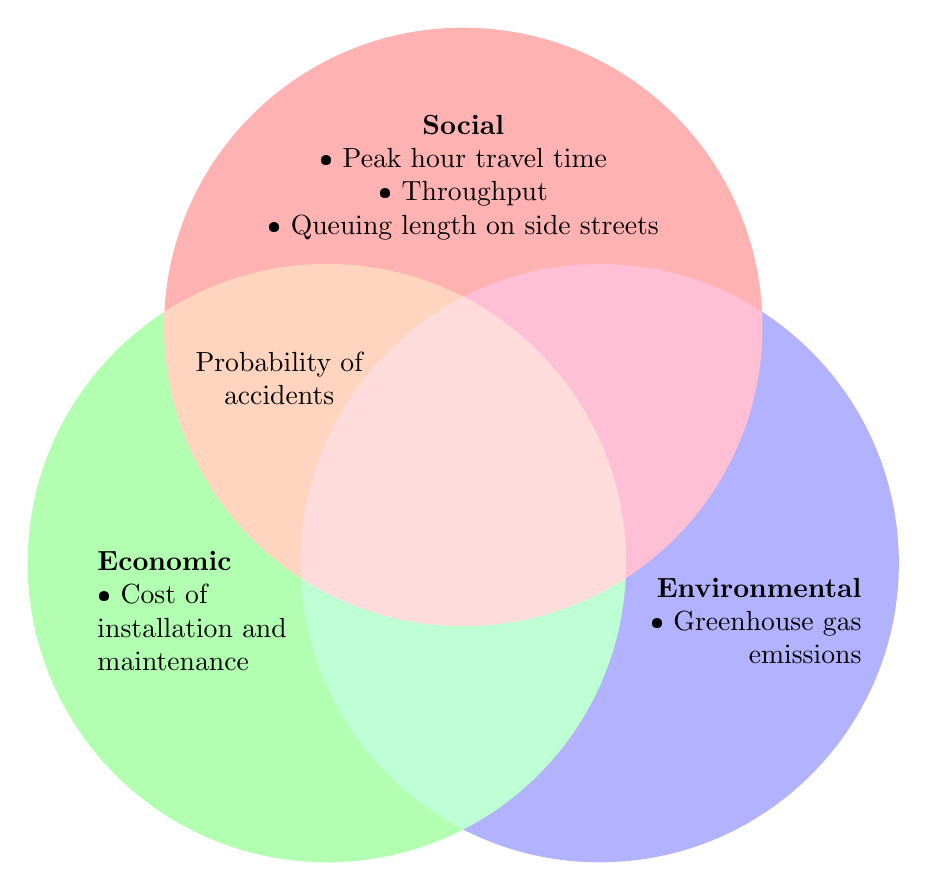
\begin{tikzpicture}
\begin{scope}[blend group = soft light]
    \fill[red!30!white]   ( 90:2) circle (3.8);
    \fill[green!30!white] (210:2) circle (3.8);
    \fill[blue!30!white]  (330:2) circle (3.8);
  \end{scope}
  \node [align=center] at  ( 90:3.9)    {\textbf{Social} \\ \textbullet\ Peak hour travel time \\ \textbullet\ Throughput \\ \textbullet\ Queuing length on side streets};
  \node [align=left] at ( 205:3.8)   {\textbf{Economic} \\ \textbullet\ Cost of\\ installation and\\ maintenance};
  \node [align=right] at ( 335:4.1)   {\textbf{Environmental} \\ \textbullet\ Greenhouse gas \\emissions};
  \node [align=center] at (150:2.7) {Probability of\\ accidents};
\end{tikzpicture}  
}
\end{figure}

%----------------------------------------------------------------------------------------
%	PROPOSED SOLUTION
%----------------------------------------------------------------------------------------

\section{Proposed Solution}

Surrey is a pioneering city when it comes to adaptive signalling so other municipalities would be interested to know whether the switch to an adaptive system is economically feasible and effective. This is especially pertinent in the Lower Mainland where population density is increasing and roads are reaching capacity, with mixed transport modes.  \\ \\
Team 7’s Synchro models and benefit-cost analysis would allow us to determine the true value of the switch to adaptive signalling from manual timed coordination and help with the decision making process, at least at a city planning level. The following scenarios are the possible outcomes from our analysis.

\subsection*{Scenario 1}
The adaptive signalling proves to add value to Surrey’s Traffic Management Centre (TMC) and should be extended to other intersections in Surrey as well as other municipalities across the province and country. This would be ideal for current stakeholders as it means that their investment in it so far is justified and effective. Surrey is one of the fastest growing cities in North America and the massive growth in road users needs urgent addressing. 

\subsection*{Scenario 2}
The adaptive signalling is seen as a net loss in value for Surrey’s TMC. This is a possibility given that some of Surrey’s Traffic engineers admitted that adaptive signalling sometimes performs worse than or just the same as the older time coordinated system. This means that their is no significant gain from switching over and the investment cannot be justified. Another challenge here is that ASCT is proprietary software with controllers based in Toronto, giving controllers in Surrey less control over the system. This will be addressed in depth in the expected challenges section.

\subsection*{Scenario 3}
The adaptive signalling works at particular intersections, but not all of them. In this case, we would identify situations in which adaptive signalling works better than manual time based coordination and recommend it only in those situations. 

%----------------------------------------------------------------------------------------
%	EXPECTED CHALLENGES
%----------------------------------------------------------------------------------------

\section{Expected Challenges}

Due to the nature of this project and the limited experience of our team, it is expected that we have to push the boundary of our expertise and face unanticipated issues. In order to prepare for these challenges, and limit delay on our work, Team 7 has identified and provided solutions to possible obstacles for this project. \\ \\
The City of Surrey is said to be the fastest growing city in British Columbia in the past decade. The rapid rate of population growth means that historical data quickly becomes obsolete. Furthermore, studies performed today will not reflect future levels of traffic flow. In order to deal with this issue, Team 7 will research how best to estimate future population growth in Surrey. A sensitivity analysis will also be conducted when analysing any future scenarios so that different levels of population growth can be compared. \\ \\
Team 7 acknowledges our team has limited experience completing a travel time study, and is unfamiliar with the process and the equipment. This equipment includes a magnet and computer logger graciously lent to us by the Surrey TMC. As this challenge has been anticipated, Team 7 has already begun researching past travel time studies so as to perform it correctly. In addition, the Surrey TMC has expressed a willingness to help with any questions or problems that may arise. \\ \\
Another issue which may impede our analysis is not being able to acquire the logic behind the adaptive signal control technology. As it is owned by another company, Delcan, the Surrey TMC does not have access to the adaptive signaling software. Our client receives real time feedback with regards to signal timing and phasing but they are not aware of the process that led to this output. Therefore, as Team 7 analyzes the adaptive control relative to the time based coordination and free flow, there will not be as full picture as to which process is superior. Also, it will be difficult to compare ASCT to other software of its type without knowledge of how it works. In response to this, Team 7 will include this limitation in our recommendations. This will also require us to provide recommendations based on output and not the signal timing process. \\ \\
Despite the possible challenges that this project entails, our team is excited to begin analyzing the 72nd Avenue corridor in Surrey. Having identified potential issues with this project, Team 7 feels confident that we can provide an insightful recommendation regarding adaptive signaling.


%----------------------------------------------------------------------------------------
%	APPENDICES
%----------------------------------------------------------------------------------------
\newpage
\newgeometry{right=1cm,bottom=1cm}
\pagenumbering{roman}
\begin{appendices}


\section{Project Report Outline}
\begin{enumerate}
\item Introduction
	\begin{enumerate}
	\item Background
	\item Policy Basis
	\item Purpose
	\item Scope
	\end{enumerate}
\item Problem
	\begin{enumerate}
	\item Issues
	\item Stakeholders
	\end{enumerate}
\item Analysis
	\begin{enumerate}
	\item Free Mode Travel Time Study
	\item Scenarios
		\begin{enumerate}
		\item Free Mode
		\item Time Based Coordination
		\item Adaptive Signalling
		\end{enumerate}
	\item Evaluation
	\end{enumerate}
\item Plan 
	\begin{enumerate}
	\item Discussion
	\item Funding Scheme
	\item Implementation Plan
	\end{enumerate}
\item Conclusion
\end{enumerate}

\end{appendices}
%----------------------------------------------------------------------------------------


\end{document}
